\chapter{User Manual}
     
\section{Hardware overview}
You can take a look of the technical data of Care-O-Bot in he official web : \url{http://www.care-o-bot-research.org/care-o-bot-3/technical-data} and \url{http://www.care-o-bot-research.org/care-o-bot-3/components}
Also you can see the distribution of the different Care-O-Bots in 
\\ \url{http://www.ros.org/wiki/Robots/Care-O-bot/distribution}

It is important an overview of the emergency stop localizations and Start/Stop key , the plugged cable of the battery and the scanners: 
\begin{center}
 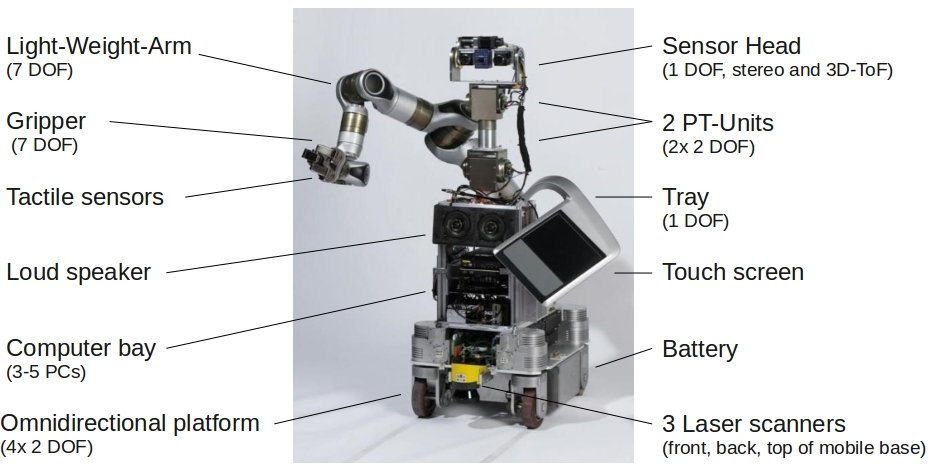
\includegraphics[width=0.95\textwidth]{images/hardware_overview.jpg}
 \end{center}

\section{Software overview} 
The bringup level repositories of Care-O-bot are the following:
\begin{itemize}
\item {cob\_extern} : The cob\_extern stack contains third party libraries needed for operating Care-O-bot. The packages are downloaded from the manufacturers website and not changed in any way.
\item {cob\_common} : The cob\_common stack hosts common packages that are used within the Care-O-bot repository. Also the URDF description of the robot, kinematics and dynamics, 3D models of robot components, information required for gazebo to simulate the COB and utility packages or common message and service definitions
\item schunk\_modular\_robotics : It is the cob\_common stack for the components of Schunk in this case lwa and sdh. 
\item cob\_driver : The cob\_driver stack includes packages that provide access to the Care-O-bot hardware through ROS messages, services and actions. E.g. for mobile base, arm, camera sensors, laser scanners, etc...
\item cob\_robots :  The cob\_robots stack collects Care-O-bot components that are used in bringing up a robot. The user's interface to the cob\_robots stack is cob\_bringup,  where are localize the launch files of the robot.
\item cob\_environments : This stack provides the parameters of the environments configuration. 
\item cob\_command\_tools: This stack provides the source code of the tools that you need to command instructions to the robot: cob\_command\_gui, cob\_dashboard, cob\_script\_server and cob\_teleop. 
\end{itemize}
\section{Batteries and Power}
Care-O-bot provides a Gaia rechargeable Li ion battery (60 Ah 48V) , in order to assure that Care-o-bot has always power it is a recommendable keep the robot plugged when it is not in use. The Power supply has to be set to 56 Volts. Before run the robot be sure that it has power.
\section{Run the robot}
First you have to connect the power supply to the robot or you can use the battery pressing the green button on the base. To switch on the robot you use the key that it has in the base , you have to move it to the position II and wait few seconds. It is recommendable stop the robot when you are not using it during some time with the emergency stop.

\begin{center}
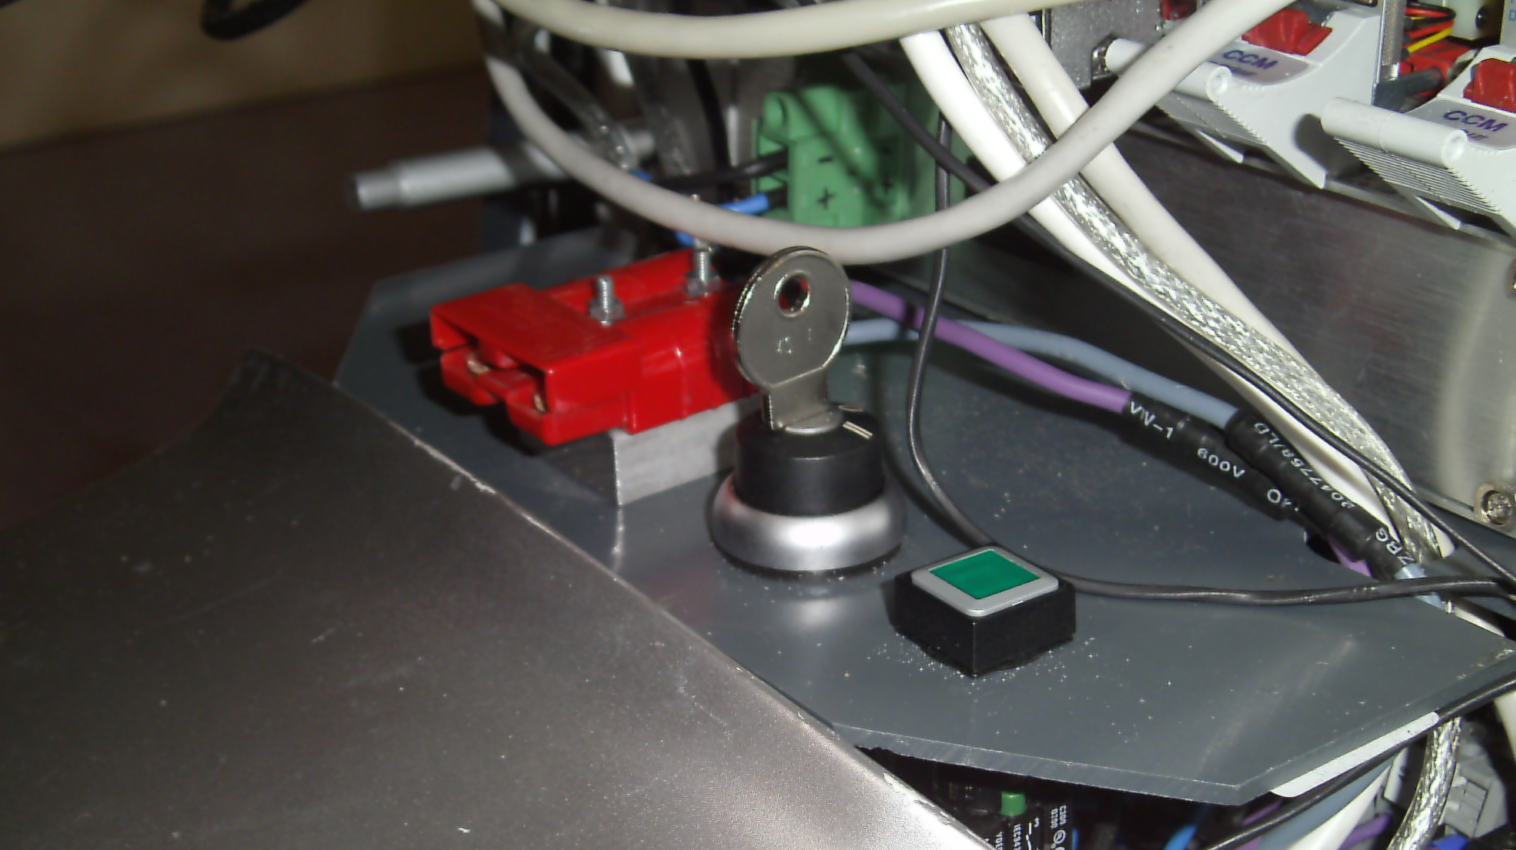
\includegraphics[width=0.3\textwidth]{images/key.png}
\end{center}
\section{Logging In}

For logging with a remote PC to the robot you have to have a account already create  (see the section 1.4) and use a secure shell connection with the PCs of the robot (it is recommended do it with executable rights).
\\
\\   \colorbox{light-gray}{
         \begin{minipage}{1.0\textwidth} 
		ssh -X user\_name@cob3-X-pcX
         \end{minipage}  } \\

\section{Bringup}

The first step to bringup the robot is the roscore, it is necessary  to have communication between the nodes. You can run it using this command: \\
\\   \colorbox{light-gray}{
         \begin{minipage}{1.0\textwidth} 
		roscore
         \end{minipage}  } \\
	\\
\\If you want to run the robot you have a launch file for launch all the components of the robot, it is localized in the package cob\_bringup, you can call this file  with the following instruction:
\\
\\   \colorbox{light-gray}{
         \begin{minipage}{1.0\textwidth} 
		roslaunch cob\_bringup robot.launch
         \end{minipage}  } \\

\section{Dashboard}
To have always under control the state of all the components of the robot you can use the tool dashboard , it is in the package cob\_bringup:
\\
\\   \colorbox{light-gray}{
         \begin{minipage}{1.0\textwidth} 
		roslaunch cob\_bringup dashboard.launch
         \end{minipage}  } \\
	\\
After this launch this file you will see in your display two windows , one is the command\_gui , where you can init , recover and move to a predefine position the different components of the robot, in the superior left corner of the command\_gui you see the current state of the robot, before move the robot , check that the status is OK. The second window is cob\_dashboard, in this windows you can see the state of Diagnostics, Motors , EM(Emergency) and Battery. In the diagnostics you have there buttons Diagnostics, rosout and Motors. 

In the case of the Care-O-bot we have disable the buttons for the Motors, you see them always in red. 

If you click the first one you will see a new window with three levels: Errors, Warnings and All. There you can see anytime the state of each component. 

\subsection {cob\_dashboard}

The dashboard is a important tool where you can check the the state of the robot, it is recommended that you have it always opened. This is the format:
\\
\begin{center}
 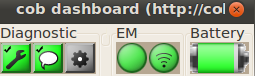
\includegraphics[width=0.55\textwidth]{images/dashboard.png}
 \end{center}
The different buttons that you have are distributed into Diagnostics, Motors, EM and Battery.

\begin{itemize}
\item Diagnosticts
\begin{itemize}
\item Diagnostics: Open the window of Diagnostics , with a list with the state of the components, the warnings and errors.
\\
 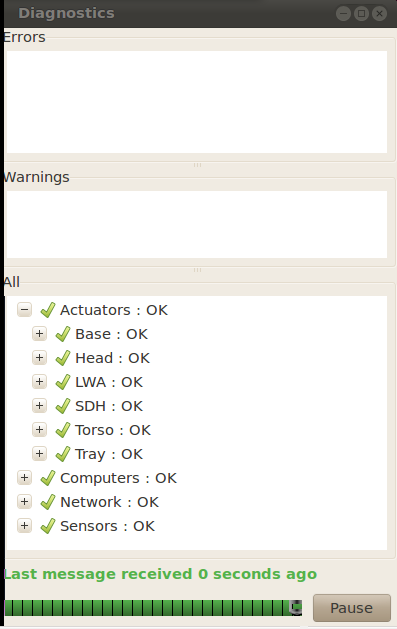
\includegraphics[width=0.45\textwidth]{images/diagnostics.png}
 \\
\item Rosout: you can check if you have communication between your nodes, it has three states OK/Error/Warm , it is determinate for the messages received the last 30 seconds.
\item Motors: it is disable for Care-O-Bot
\end{itemize}
\item Motors : These buttons are disable.
\item EM : In this display you can see the state, if it is red the emergency stop is activated if not it is green.
\item Battery: you can see the state of the battery , green : full, orange : 40\% and red 20\%
\end{itemize}

\subsection {Diagnostics}

\subsection{cob\_command\_gui}
The standard view of the command\_gui is:
\\
\\
 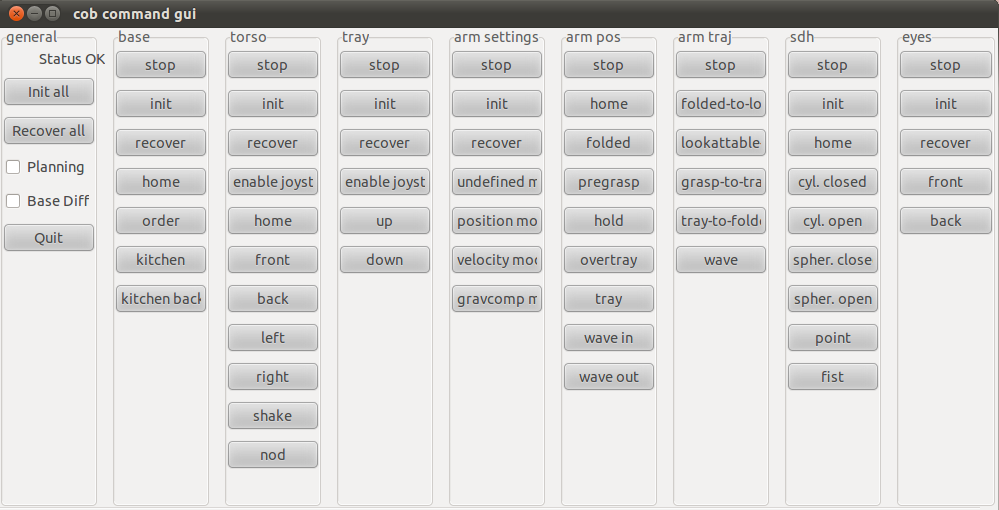
\includegraphics[width=1\textwidth]{images/cob_command_gui.png}
\\
\\
In this screenshot you can see different columns:  general, base, torso, tray, arm settings, arm pos, arm traj, sdh and eyes.

The first column is very important , when you run the robot, if you want to move it, the first that you have to do is click "init all" you will see in the window dashboard the initialization of each component, after a Emergency stop you have to press the button "recover all", the columns of the components have different predefine positions , you can change it in the configuration when you want , also each component has a "stop", "init" and "recover" button , when you see that you have an error in only one of these components you can press only "recover" for this one.

\section{Rviz}
RVIZ is a program that visualizes additional views to the robot e.g. the original images from the camera, the path where the Care-O-bot is moving to and many more. You can add your own items to RVIZ to visualize topics. You can see more information in \url{http://www.ros.org/wiki/rviz}
You can communicate the robot with your local PC and execute RVIZ in it:
\\
\\   \colorbox{light-gray}{
         \begin{minipage}{1.0\textwidth} 
		export ROS\_MASTER\_URI=http://cob3-3-pc1:11311
		\\rosrun rviz rviz
         \end{minipage}  } \\
	\\


You will see a screen like this:
\begin {center}
 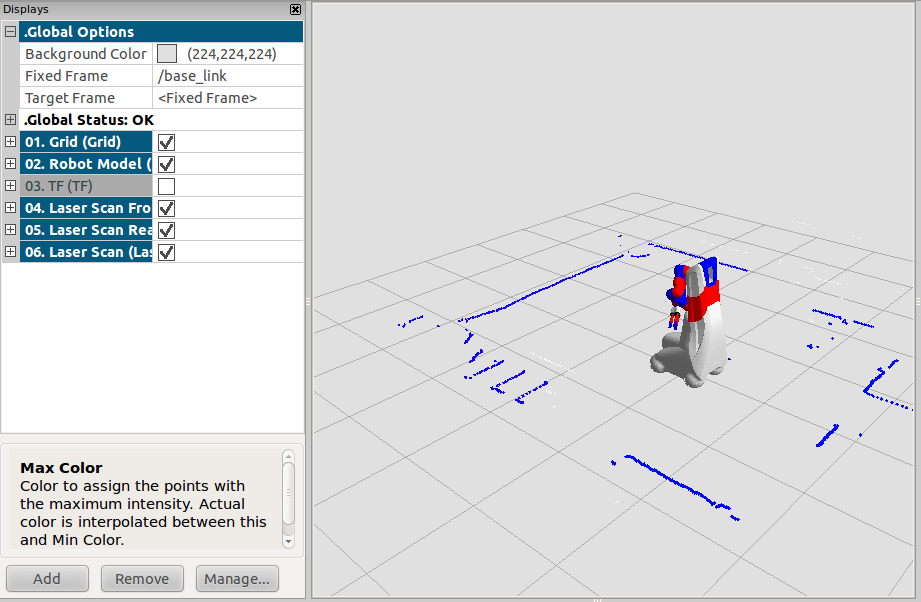
\includegraphics[width=1\textwidth]{images/rviz.png}
\end{center}
If you see that the robot is not in the same position in the real environment than in Rviz you have to localize it using  the buttons of Rviz 2D Nav Goal  and 2D Pose Estimate

\section{Joystick}
To be able to use the joystick the deadman\_button has to be pressed all the time, as soon as the button is released a stop will be send to all hardware components. 

\begin{itemize}
\item For moving the base: Hold the deadman button and use the base rotation and translation axis to move the base.

\item For moving the torso: Hold the deadman button and the upper or lower neck button, then use the up\_down or left\_right axis to move the torso.

\item For moving the tray: Hold the deadman button and the tray button, then use the up\_down axis to move the tray.

\item For moving the arm: Hold the deadman button and one of the arm buttons, then use the up\_down or left\_right axis to move the selected arm joints.
\end{itemize}

Have a look at the following image to see which buttons command which components. 

\begin{center}
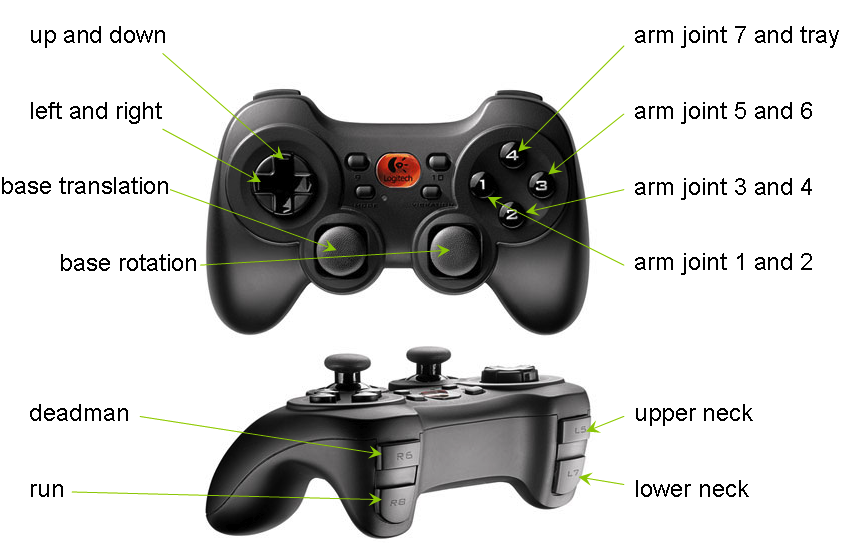
\includegraphics[width=1\textwidth]{images/joystick.png}
\end{center}

\section{Emergency stop} 
The user has two possibilities to activate the EM Stop, on the robot you have two red buttons on the laterals you press it when you see that the Care-O-Bot will have an accident. The second possibility is with the Remote, you have to hold this remote control on your hand always that you move Care-O-Bot. 
\subsection{Emergency stop remote control}

You can press the red button to stop the robot, after a emergency stop you have to restart the computers, to do it you have to be sure that you have already "up" all the red-emergency stop buttons, the press the green button of the Remote control and then move again the key of the robot to the II position. You will see on your remote PC a message "Emergency stop released!", the you have to press "recover all" in the on the command\_gui , open Diagnostics and check that all components are green. 

\begin{center}
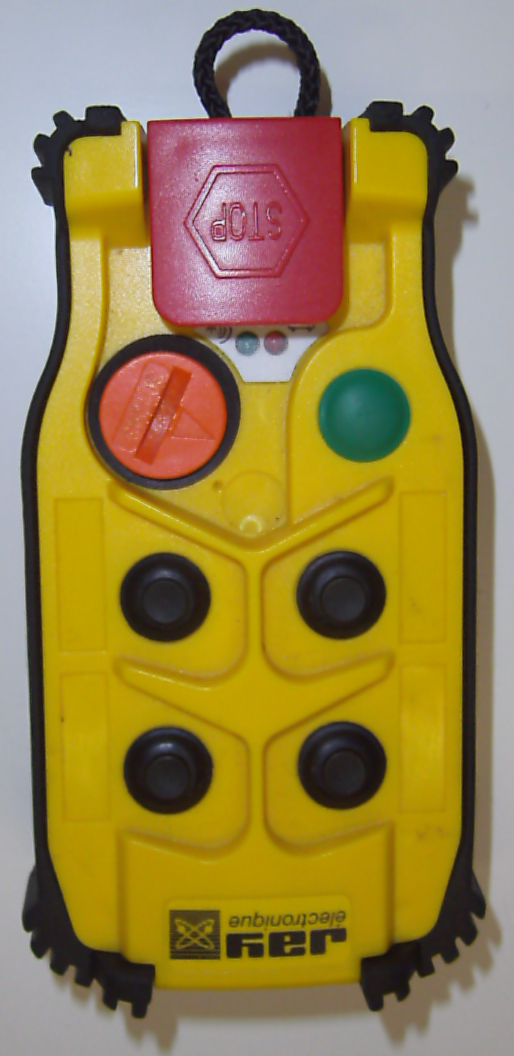
\includegraphics[width=0.15\textwidth]{images/em_stop.png}
\end{center}

\section{Putting away}
You have to logout in the local PC (Ctrl+D) and press the emergency stop, then you can shut down the PCs, moving the key to the position I (left).
\section{Support}
If you have doubts , please use our Mainlist : \url{http://www.care-o-bot-research.org/contributing/mailing-lists}
\section{Packing-Shipping} 
